\section{Startup, Operating Modes, and Shutdown}
\label{sec:ctrl-state}

Secondary-side power may be unavailable at startup, so PA1 feedback cannot be assumed valid immediately after \texttt{ON}. Precharge alternates bounded energy packets and inhibited settling intervals before checking readiness.

The default request is \SI{0.1}{\percent} average duty for \SI{3}{\milli\second}, followed by \SI{80}{\milli\second} settling. Up to four bursts are allowed, with a \SI{4}{\volt} readiness threshold. The actual bursts are still determined by the minimum enabled intervals and pulse skipping.

\begin{figure}[htbp]
\centering
\begingroup
\definecolor{ctrlnavy}{HTML}{153448}
\definecolor{ctrlteal}{HTML}{007C83}
\definecolor{ctrlred}{HTML}{990000}
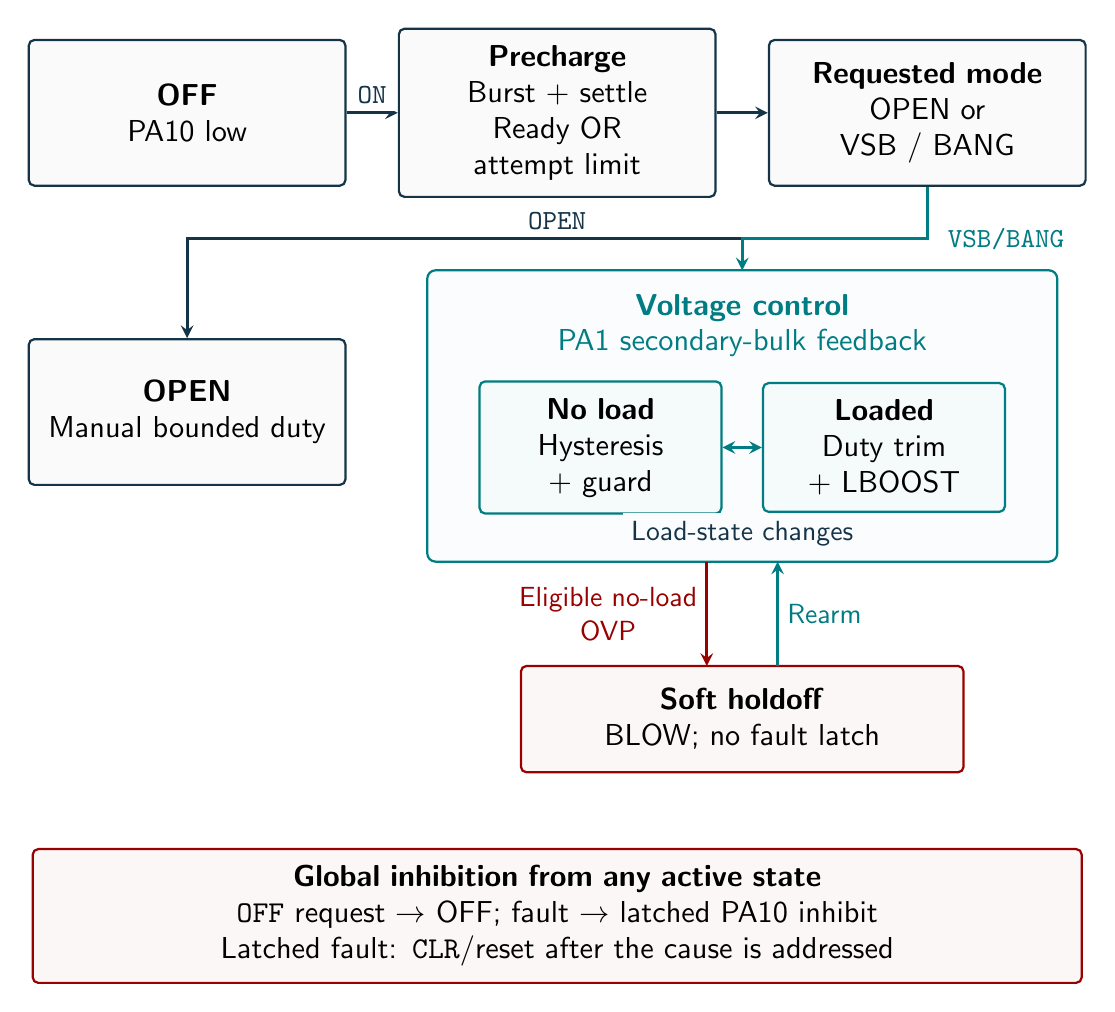
\begin{tikzpicture}[
font=\sffamily\fontsize{11}{13}\selectfont,
every node/.style={align=center,inner sep=6pt,
    execute at begin node={\hyphenpenalty=10000\exhyphenpenalty=10000}},
state/.style={draw=ctrlnavy,fill=black!2,rounded corners=2pt,
    line width=0.8pt,text width=3.6cm,minimum height=1.85cm},
run/.style={state,draw=ctrlteal,fill=ctrlteal!4},
hold/.style={state,draw=ctrlred,fill=ctrlred!3,minimum height=1.35cm},
flow/.style={->,>=stealth,draw=ctrlnavy,line width=1.0pt},
runflow/.style={flow,draw=ctrlteal},
inhibit/.style={flow,draw=ctrlred},
annotation/.style={font=\sffamily\fontsize{10}{12}\selectfont,text=ctrlnavy,
    inner sep=3pt,fill=white}]
\node[state] (off) at (0,0) {\textbf{OFF}\\PA10 low};
\node[state] (pre) at (4.7,0)
    {\textbf{Precharge}\\Burst + settle\\Ready OR attempt limit};
\node[state] (mode) at (9.4,0)
    {\textbf{Requested mode}\\OPEN or\\VSB / BANG};
\node[state] (open) at (0,-3.8)
    {\textbf{OPEN}\\Manual bounded duty};
\draw[draw=ctrlteal,fill=ctrlteal!2,rounded corners=3pt,line width=0.8pt]
    (3.05,-2.0) rectangle (11.05,-5.7);
\node[text=ctrlteal] at (7.05,-2.7)
    {\textbf{Voltage control}\\PA1 secondary-bulk feedback};
\node[run,text width=2.65cm,minimum height=1.4cm] (light) at (5.25,-4.25)
    {\textbf{No load}\\Hysteresis + guard};
\node[run,text width=2.65cm,minimum height=1.4cm] (loaded) at (8.85,-4.25)
    {\textbf{Loaded}\\Duty trim + LBOOST};
\node[annotation,fill=ctrlteal!2] at (7.05,-5.35) {Load-state changes};
\node[hold,text width=5.2cm] (soft) at (7.05,-7.7)
    {\textbf{Soft holdoff}\\BLOW; no fault latch};
\node[hold,text width=12.9cm,minimum height=1.6cm] at (4.7,-10.2)
    {\textbf{Global inhibition from any active state}\\
    \texttt{OFF} request $\rightarrow$ OFF; fault $\rightarrow$ latched PA10 inhibit\\
    Latched fault: \texttt{CLR}/reset after the cause is addressed};
\draw[flow] (off) -- node[annotation,above] {\texttt{ON}} (pre);
\draw[flow] (pre) -- (mode);
\draw[flow] (mode.south) -- (9.4,-1.6) --
    node[annotation,above] {\texttt{OPEN}} (0,-1.6) -- (open.north);
\draw[runflow] (mode.south) -- (9.4,-1.6) -- (7.05,-1.6) -- (7.05,-2.0);
\node[annotation,text=ctrlteal,anchor=west] at (9.55,-1.6) {\texttt{VSB/BANG}};
\draw[runflow,<->] (light) -- (loaded);
\draw[inhibit] (6.6,-5.7) -- node[annotation,left,text=ctrlred]
    {Eligible no-load\\OVP} (6.6,-7.025);
\draw[runflow] (7.5,-7.025) -- node[annotation,right,text=ctrlteal]
    {Rearm} (7.5,-5.7);
\end{tikzpicture}
\endgroup
\caption{Baseline firmware states. OPEN selects manual duty; voltage control switches between loaded and no-load operation and can enter soft holdoff at \texttt{BLOW} (default zero). OFF and latched faults force PA10 low.}
\label{fig:ctrl-state-diagram}
\end{figure}

\begin{table}[htbp]
\centering
\caption{Firmware states, actions, and exit conditions.}
\label{tab:ctrl-state-machine}
\begin{tabularx}{\textwidth}{@{}p{0.22\textwidth}Xp{0.29\textwidth}@{}}
\toprule
State & Action & Exit condition\\
\midrule
OFF & Configure peripherals and hold PA10 low & Valid \texttt{ON} request\\
Precharge & Alternate small energy packets and settling & Readiness threshold or attempt limit, OFF, or fault\\
OPEN & Apply the operator's bounded enable command & Mode change, OFF, or fault\\
Voltage control & Use PA1 thresholds with loaded/no-load behavior & Mode change, OFF, or fault\\
Soft holdoff & Request \texttt{BLOW} (default zero) without latching & Voltage reaches rearm condition, OFF, or fault\\
Fault latched & Inhibit PA10 & \texttt{CLR} or reset after the cause is addressed\\
\bottomrule
\end{tabularx}
\end{table}

Startup proceeds when \texttt{PREV} is reached \emph{or} \texttt{PREMAX} is exhausted. Exhausting attempts does not itself latch a dedicated startup fault. Other fault checks remain active. A timed startup trace must therefore include feedback voltage and state to show why normal operation began.

\texttt{OPEN} selects manual duty; \texttt{VSB}/\texttt{BANG} selects voltage control. Runtime enable is separate from \texttt{BOOTON}/\texttt{BOOTOFF}, which save the boot preference. \texttt{OFF} inhibits transfer. Any charge in the link and output capacitors remains until discharged through the available paths.
